\documentclass[twoside]{article} 
\usepackage{geometry}
\geometry{verbose,a4paper,tmargin=1.5cm,bmargin=1.5cm,lmargin=1.5cm,rmargin=1.5cm}
\usepackage{graphicx}



\begin{document}
\fbox{ {\large
    \begin{tabular}[t]{lcr}
      \begin{minipage}{2in}
        \begin{center}
          Master M1 Informatique
        \end{center}
      \end{minipage} & 

      \begin{minipage}{2in}
        \begin{center}
          BattleShip2D\\
	 User manual
        \end{center}
      \end{minipage} &

      \begin{minipage}{2in}
        \begin{center}
          X. Skapin\\
        \end{center}
      \end{minipage}
    \end{tabular}
  }} \vspace*{.5cm}

\tableofcontents

\section{Presentation}
\textbf{BattleShip2D} is a Java-FX game to play to the classic BattleShip in graphical version: one human user plays versus the computer and each protagonist targets the cell of the other one, every turn. 
The winner is the first protagonist which has destroyed the entire fleet of opponent's vessels.

\section{Contents}
This file is part of the \textbf{BattleShip2D} project, made of:
\begin{itemize}
\item \textit{Documentation}: provides
\begin{itemize}
\item this file, both in \LaTeX\  and PDF formats;
\item \textit{doxyfile}, the \texttt{Doxygen} configuration file used to produce code documentation in HTML. In order to get drawings of classes relationships, the \textbf{Graphviz} package is required.
\item \textit{html} and \textit{latex} directories, resulting from running \texttt{Doxygen}.
\item \textit{figures}, grouping images used in this document.
\end{itemize}
\item the \textit{META-INF} directory used to create \textit{BattleShip2D.jar}
\item the \textit{COPYING} file provided to comply to GPL3 license
\item the jar archive named \textit{BattleShip2D.jar}. Besides the code classes, this archive contains the source code of the \texttt{model} package. 
\item \textit{README.TEXT}, a short notice about the project's contents.
\end{itemize}

\section{Code documentation}
Both \textit{html} and \textit{latex} directories should contain the complete project code documentation (either in HTML or \LaTeX\ formats), resulting from running \texttt{Doxygen} on the \textit{doxyfile} file. However, if this directory either does not exist or is empty, you can re-create the documentation files by running:
\begin{verbatim}
$ doxygen
\end{verbatim}


\section{Source code compilation}

This manual should be provided in the directory \textit{BattleShip2D}. This directory should also contain Java files located in the subdirectory \texttt{battleship2d}. WARNING: the subdirectory \texttt{battleship2D/ui} only contains classes but no \texttt{JavaFX} code.\\

Before compiling, make sure that \texttt{Java~8} has been properly installed on your computer. 
\begin{enumerate}
\item One way to know your version of \texttt{java}\footnote{The procedure is the same for \texttt{javac} is to type (under \texttt{Debian}-like systems)}:
\begin{verbatim}
$ java -version
\end{verbatim}
\item Some systems may have several different versions of \texttt{Java}. Type the following commands to list them:
\begin{verbatim}
$ update-alternatives --config java
\end{verbatim}
\item If \texttt{Java~8} is actually in the list but is not selected as actually the used version, the system offers you to select the valid version (you may need to be logged as \textit{root}).
\item Once you have the valid versions of both \texttt{java} and \texttt{javac}, go into the directory \textit{BattleShip2D} and run the compilation as follows:
\begin{verbatim}
$ javac -Xlint:all battleship2d/model/*.java
\end{verbatim}

\item You can also (re)create the jar archive \textit{BattleShip2D.jar} as follows:
\begin{verbatim}
$ jar cmvf META-INF/MANIFEST.MF BattleShip2D.jar META-INF battleship2d/*
\end{verbatim}

\end{enumerate}

\section{Playing BattleShip2D}

The objective for the player is to place its ships on its game board, then play against the computer to destroy the opponent's ships.

\subsection{Overview}

Run \textit{BattleShip2D.jar} by typing:
\begin{verbatim}
$ java -jar BattleShip2D.jar
\end{verbatim}

or move to the \texttt{battleship2D}'s parent directory and type:
\begin{verbatim}
$ java battleship2D.ui.BattleShip2D
\end{verbatim}


The main windows are displayed (fig.~\ref{fig:mainWindows01}). 
\begin{itemize}
\item On the top-left part, the players's board is displayed as a 10x10 empty game board. Each cell is currently empty, with an ocean background.
\item On the top-right part, the computer's game bord is currently hidden, until the player has positioned its fleet of ships. 
\item The bottom part is made of two panels: one for selecting the ships to position on the board, the other for displaying game information.
The first panel is a choice box, providing information about fleet ships:
\begin{itemize}
\item Name (\textbf{CARRIER}, \textbf{BATTTLESHIP}, \textbf{CRUISER}, \textbf{DESTROYER}, \textbf{SUBMARINE})
\item Size in cells (\textbf{5}, \textbf{4}, \textbf{3}, \textbf{2}, \textbf{1})
\item the \texttt{Done} button is used to valid ship insertion. The computer's board is displayed as soon as every player's ship has been positioned (an error message is displayed if the button is pushed while some ships have not been positioned).
\end{itemize}
\end{itemize}

\begin{figure}[h!]
\centering
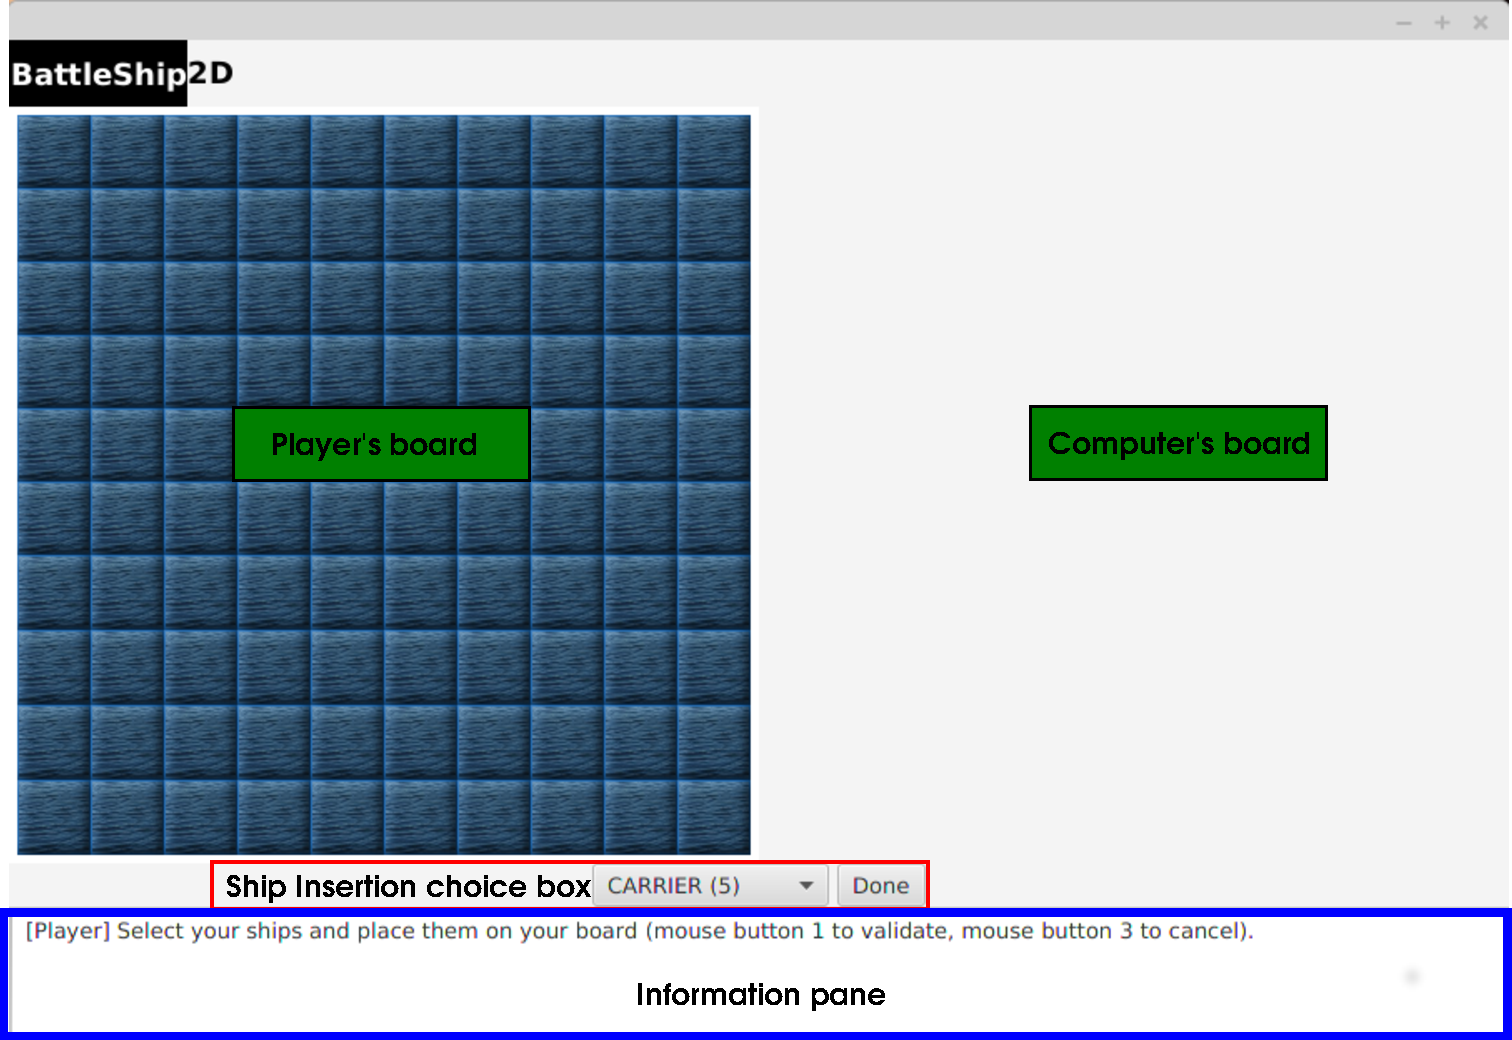
\includegraphics[scale=0.45]{figures/mainWindowsDescription-01.pdf}
\caption{Description of game windows}
\label{fig:mainWindows01}
\end{figure}


\subsection{Positioning the player's ships}


The \textbf{Information} panel at the very bottom of the application prompts dynamic messages.
\begin{enumerate}
\item The first message is:
\begin{verbatim}
[Player] Select your ships and place them on your board (mouse button 1 to validate,
mouse button 3 to cancel). 
\end{verbatim}
\end{enumerate}

\begin{enumerate}
\item[2.] Inserting a ship follows a 4-step procedure, described in fig.~\ref{fig:insertingShip}. The set of available cells for every ship depends on the location of the center cell (selected by clicking on it) and the ship already placed on the board. Use the Ship insertion choice box to select the kind of ship you want. It is possible to change the position of a ship already placed on the board. And remember that clicking on the mouse button 3 cancels the last ship insertion.
\end{enumerate}

\begin{figure}[h!]
\centering$
\begin{array}{cc}
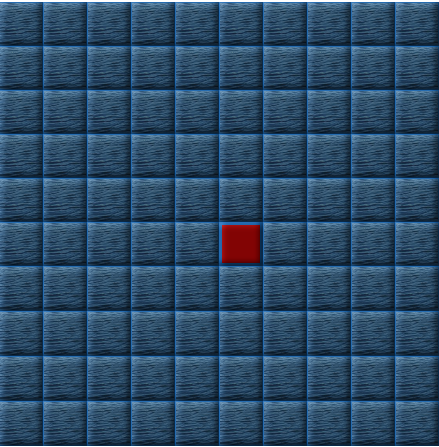
\includegraphics[scale=0.4]{figures/shipInsertion-01.png} & 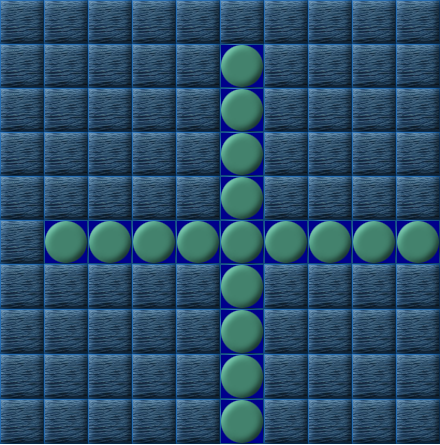
\includegraphics[scale=0.4]{figures/shipInsertion-02.png}\\
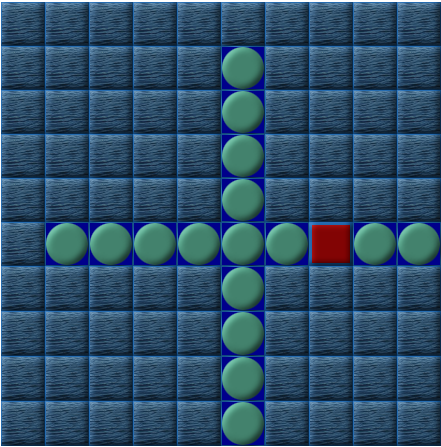
\includegraphics[scale=0.4]{figures/shipInsertion-03.png} & 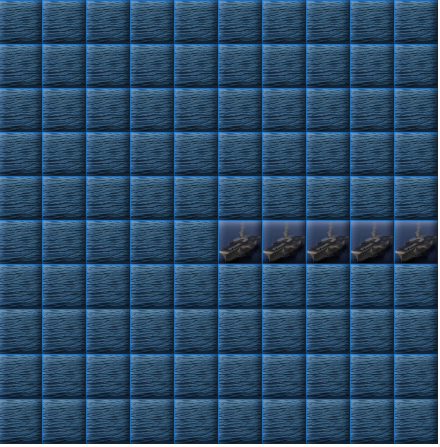
\includegraphics[scale=0.4]{figures/shipInsertion-04.png}
\end{array}$

\caption{Ship insertion. From top-left to bottom-right: the cell under the mouse is marked in red; after clicking, the cells available to position a ship are displayed along the four cardinal orientations; hovering the mouse on a available cell allows to choose an orientation; clicking once again inserts the current ship.}
\label{fig:insertingShip}
\end{figure}


\newpage

\subsection{Playing against the computer}

\begin{enumerate}
\item[1.] Once all the ships have been inserted, click on the button "\texttt{Done}"\footnote{This button does nothing while there is at least one ship to insert (and a warning message is displayed in the information pane).} next to the choice box. The computer's board is diaplayed, with every cell shown in black to hide its ships (fig.~\ref{fig:allShipsInserted}). A message in the information pane prompts you to select a cell on the computer side.
\end{enumerate}

\begin{figure}[h!]
\centering
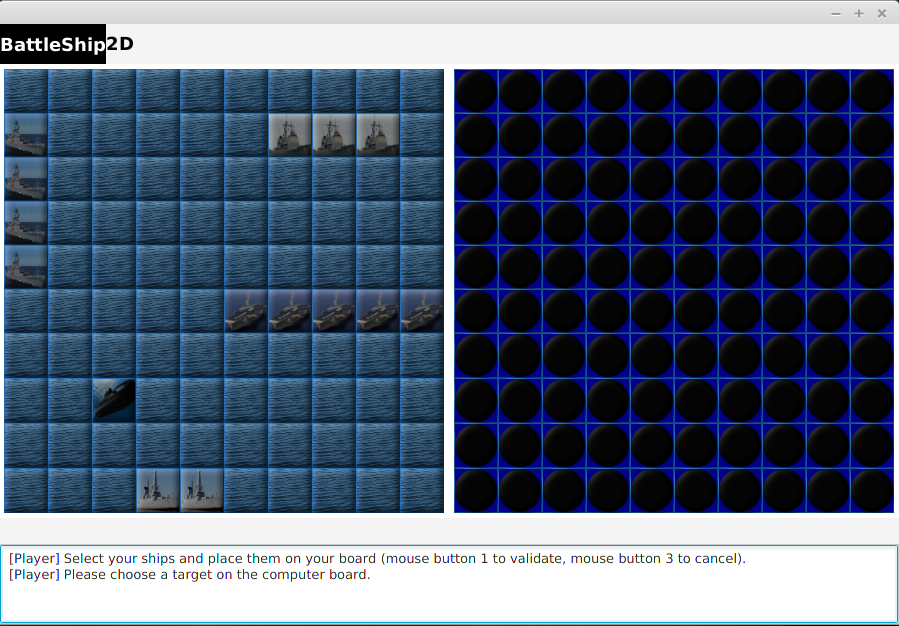
\includegraphics[scale=0.65]{figures/allShipsInserted.png}
\caption{The game is ready to start.}
\label{fig:allShipsInserted}
\end{figure}

\begin{enumerate}
\item[2.] Once a cell has been clicked on the computer side, a missile (displayed as an orange sphere) is launched from one of the player's ships\footnote{The ship is randomly chosen each time. More precisely, the missile is launched from one of the cell filled with an image ship that has not been hit.}, as shown in fig.~\ref{fig:missileLaunch}.
\end{enumerate}

\begin{figure}[h!]
\centering
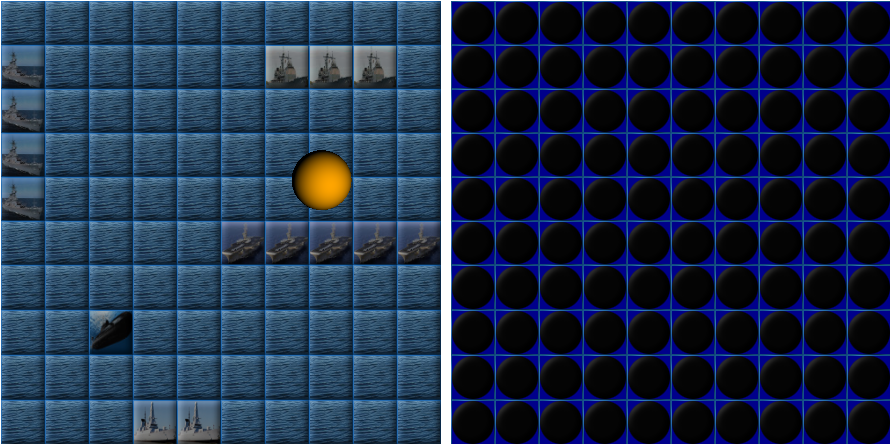
\includegraphics[scale=0.65]{figures/missileLaunch.png}
\caption{The first missile is launched.}
\label{fig:missileLaunch}
\end{figure}

\begin{enumerate}
\item[3.] The computer fires back with its own missile, and the game turns alternate between player and computer moves. If the missile hit only water, an "ocean" cell is displayed on the computer side. If a ship has been hit, an image of a burning ship is displayed, as shown in fig.~\ref{fig:hitShip} on the computer side, after somme unsuccessful attempts from the player. A message is displayed in the information pane each time a ship has been hit.

The computer plays with a configurable level of expertises, ranging from shooting at randomly cells to select areas next to hit ships on the player side.
\end{enumerate}

\begin{figure}[h!]
\centering
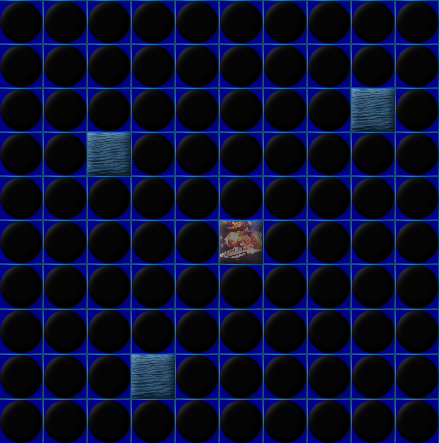
\includegraphics[scale=0.45]{figures/hitShip.png}
\caption{A ship has been hit on the computer side.}
\label{fig:hitShip}
\end{figure}


\begin{enumerate}
\item[4.] The game stops as soon as one of the opponents has destroyed all the ships of its adversary. A last animation with the name of the winner is run as soon as the last ship has been destroyed (fig.~\ref{fig:endOfGame}).
\end{enumerate}

\begin{figure}[h!]
\centering$
\begin{array}{c}
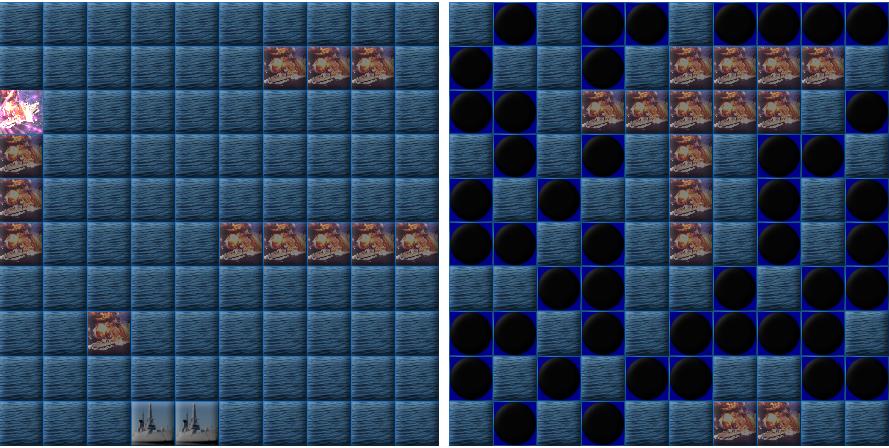
\includegraphics[scale=0.45]{figures/almostEndGame.png} \\
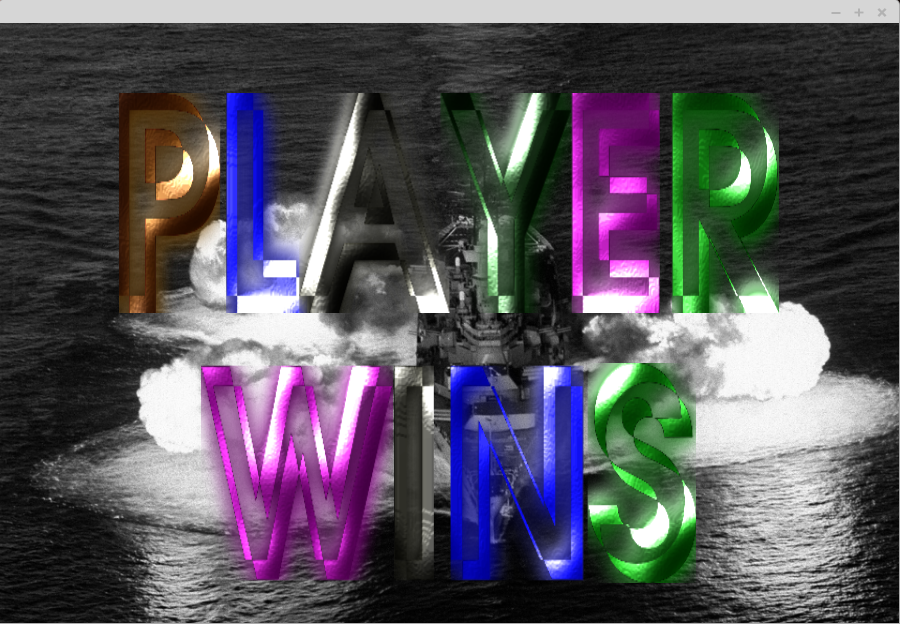
\includegraphics[scale=0.45]{figures/playerWins.png}
\end{array}$
\caption{Top: the game is almost finished: the player is still looking for the computer's submarine while its only intact ship is a two-cell sized destroyer. Bottom: the player has touched the computer's submarine and wins the game.}
\label{fig:endOfGame}
\end{figure}

\end{document}
